\documentclass[tikz,border=5pt]{standalone}
\usepackage{amsmath}
\usetikzlibrary{arrows.meta}

\definecolor{ink}{HTML}{273442}
\definecolor{spectral}{HTML}{285E8A}
\definecolor{surface}{HTML}{14756C}

% Compile with pdflatex; include the resulting PDF with \includegraphics.
% Caption: Fixed G0 + G1 plus a sum of learned, parallel filter--multiply--filter
% branches. Surface features are shared; branch-specific linear heads produce a_b.
% Each of eight multiplier networks produces 320 real Fourier weight vectors.
% FFT/IFFT denote real transforms. Normalization and min(h,5) clipping are omitted.
% The code sums branch spectra before the final IFFT within each group; drawing
% that IFFT per branch is algebraically equivalent by linearity.
\begin{document}
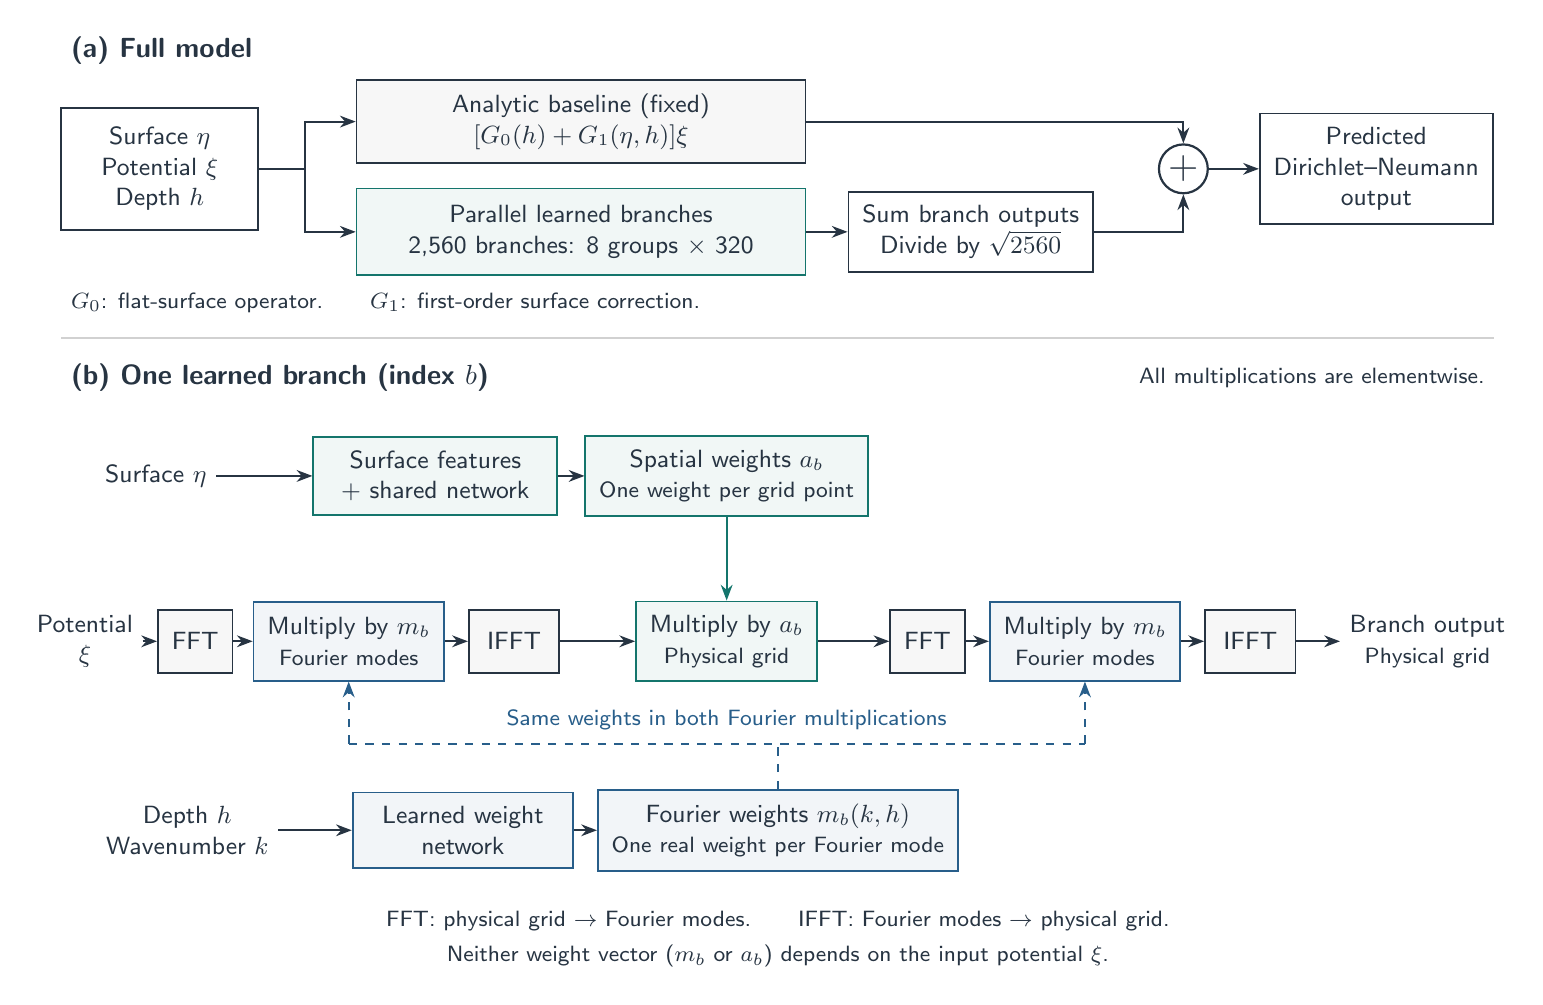
\begin{tikzpicture}[
  font=\sffamily\small, text=ink,
  block/.style={draw=ink, line width=.65pt, align=center, inner sep=5pt},
  transform/.style={block, fill=black!3, minimum height=.8cm},
  fourier/.style={block, draw=spectral, fill=spectral!6},
  spatial/.style={block, draw=surface, fill=surface!6},
  arrow/.style={-{Stealth[length=2mm]}, draw=ink, line width=.7pt},
  weights/.style={draw=spectral, dashed, line width=.8pt},
  weightarrow/.style={weights, -{Stealth[length=2mm]}},
  heading/.style={anchor=west, font=\sffamily\bfseries},
  note/.style={font=\sffamily\footnotesize, align=center}
]

% Full model: the analytic and learned paths receive the same inputs.
\node[heading] at (0,0) {(a) Full model};
\node[block, minimum width=2.5cm, minimum height=1.55cm] (inputs) at (1.25,-1.5)
  {Surface $\eta$\\Potential $\xi$\\Depth $h$};
\node[block, fill=black!3, minimum width=5.7cm, minimum height=1cm]
  (baseline) at (6.6,-.9)
  {Analytic baseline (fixed)\\$[G_0(h)+G_1(\eta,h)]\xi$};
\node[spatial, minimum width=5.7cm, minimum height=1.1cm]
  (branches) at (6.6,-2.3)
  {Parallel learned branches\\2,560 branches: 8 groups $\times$ 320};
\node[block, minimum width=2.7cm, minimum height=1cm] (sum) at (11.55,-2.3)
  {Sum branch outputs\\Divide by $\sqrt{2560}$};
\node[circle, draw=ink, line width=.8pt, minimum size=.62cm, inner sep=0pt]
  (add) at (14.25,-1.5) {\Large $+$};
\node[block, minimum width=2.8cm, minimum height=.85cm] (prediction) at (16.7,-1.5)
  {Predicted\\Dirichlet--Neumann\\output};
\draw[arrow] (inputs.east) -- (3.1,-1.5) |- (baseline.west);
\draw[arrow] (3.1,-1.5) |- (branches.west);
\draw[arrow] (baseline.east) -| (add.north);
\draw[arrow] (branches.east) -- (sum.west);
\draw[arrow] (sum.east) -| (add.south);
\draw[arrow] (add.east) -- (prediction.west);
\node[note, anchor=west] at (0,-3.2)
  {$G_0$: flat-surface operator.\qquad $G_1$: first-order surface correction.};
\draw[black!18, line width=.5pt] (0,-3.65) -- (18.2,-3.65);

% One branch: every transform and every elementwise product is explicit.
\node[heading] at (0,-4.15) {(b) One learned branch (index $b$)};
\node[note, anchor=east] at (18.2,-4.15) {All multiplications are elementwise.};
\node[align=center] (eta) at (1.2,-5.4) {Surface $\eta$};
\node[spatial, minimum width=3.1cm, minimum height=.9cm] (features) at (4.75,-5.4)
  {Surface features\\+ shared network};
\node[spatial, minimum width=3cm, minimum height=1cm] (a) at (8.45,-5.4)
  {Spatial weights $a_b$\\\footnotesize One weight per grid point};
\draw[arrow] (eta.east) -- (features.west);
\draw[arrow] (features.east) -- (a.west);

\node[align=center] (xi) at (.3,-7.5) {Potential\\$\xi$};
\node[transform, minimum width=.85cm] (fft1) at (1.7,-7.5) {FFT};
\node[fourier, minimum width=1.65cm, minimum height=1cm] (m1) at (3.65,-7.5)
  {Multiply by $m_b$\\\footnotesize Fourier modes};
\node[transform, minimum width=1.15cm] (ifft1) at (5.75,-7.5) {IFFT};
\node[spatial, minimum width=2cm, minimum height=1cm] (product) at (8.45,-7.5)
  {Multiply by $a_b$\\\footnotesize Physical grid};
\node[transform, minimum width=.85cm] (fft2) at (11,-7.5) {FFT};
\node[fourier, minimum width=1.65cm, minimum height=1cm] (m2) at (13,-7.5)
  {Multiply by $m_b$\\\footnotesize Fourier modes};
\node[transform, minimum width=1.15cm] (ifft2) at (15.1,-7.5) {IFFT};
\node[align=center] (output) at (17.35,-7.5)
  {Branch output\\\footnotesize Physical grid};
\draw[arrow] (xi.east) -- (fft1.west);
\draw[arrow] (fft1.east) -- (m1.west);
\draw[arrow] (m1.east) -- (ifft1.west);
\draw[arrow] (ifft1.east) -- (product.west);
\draw[arrow] (product.east) -- (fft2.west);
\draw[arrow] (fft2.east) -- (m2.west);
\draw[arrow] (m2.east) -- (ifft2.west);
\draw[arrow] (ifft2.east) -- (output.west);
\draw[arrow, draw=surface] (a.south) -- (product.north);

% The same coefficient vector feeds both Fourier-space multiplications.
\node[align=center] (kh) at (1.6,-9.9) {Depth $h$\\Wavenumber $k$};
\node[fourier, minimum width=2.8cm, minimum height=.9cm] (network) at (5.1,-9.9)
  {Learned weight\\network};
\node[fourier, minimum width=3.9cm, minimum height=1cm] (m) at (9.1,-9.9)
  {Fourier weights $m_b(k,h)$\\\footnotesize One real weight per Fourier mode};
\draw[arrow] (kh.east) -- (network.west);
\draw[arrow] (network.east) -- (m.west);
\draw[weights] (m.north) -- (9.1,-8.8);
\draw[weights] (3.65,-8.8) -- (13,-8.8);
\draw[weightarrow] (3.65,-8.8) -- (m1.south);
\draw[weightarrow] (13,-8.8) -- (m2.south);
\node[note, text=spectral] at (8.45,-8.5)
  {Same weights in both Fourier multiplications};

\node[note] at (9.1,-11.05)
  {FFT: physical grid $\rightarrow$ Fourier modes.\qquad
   IFFT: Fourier modes $\rightarrow$ physical grid.};
\node[note] at (9.1,-11.5)
  {Neither weight vector ($m_b$ or $a_b$) depends on the input potential $\xi$.};
\end{tikzpicture}
\end{document}
